\documentclass[a4paper,10pt]{article}
\usepackage[utf8]{inputenc}

\usepackage{amssymb,array,delarray,verbatim,alltt,epsfig,float,amsthm}
\usepackage{graphicx,algorithmicx,algorithm,algpseudocode,xspace,xcolor}
\usepackage{url}
\usepackage{listings}
\usepackage{epsf,epsfig,subfigure,dsfont}
\usepackage{amssymb,amsmath}
\usepackage{pgf,amsbsy,amsfonts,amsmath,subfigure,multicol,natbib}
\usepackage{graphicx,xspace,color,cancel}
\usepackage{tikz}
\usepackage{pythonhighlight}
\usepackage{mathrsfs}
\newcommand{\dom}[1]{\textrm{dom}\!\br{#1}}

% Title Page
\title{Assignment 2}
\author{Machine Learning Applications, Fall 2019}
\date{}


\begin{document}
\maketitle

% \begin{abstract}
% \end{abstract}
\begin{itemize}
 \item You should solve your exercises using a Jupyter Notebook (some exercises require coding).  In some exercises, it is requested that you write all the analytical steps that you made in order to get to the solution, so in this case you should write the steps using latex formulas in a Markdown cell.
 \item Solutions should be uploaded to Sulis before the due date; they should be each a single PDF document (so export your notebook to PDF), and additional files will not be considered.
\item  Students may (and should) collaboratively discuss the  assignments; however, I expect each student to write and upload their own solutions. Please write your full name and the names of the students (if any) you discussed the  assignment with at the top of your solutions.
\end{itemize}

\newpage 
\section*{Exercise 1 (points 2)}
 A \textbf{Markov Chain} (MC) is a graph whose edges are weighted with positive probabilities. The nodes the possible states of some process or machine. The probability on an edge from state A to state B is equal to the probability that the next state will be B if the current state is A. Since there must always be a next state, the sum of the probabilities leaving a node must be 1. \\~\\
 \begin{center}
  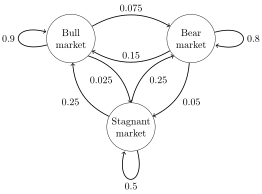
\includegraphics[width=5.5cm]{MC.png}
 \end{center}
 Consider the example in Figure from Wikipedia. 
 The states represent whether a hypothetical stock market is exhibiting a ``bull market'', ``bear market'', or ``stagnant market'' trend during a given week. According to the figure, a bull week is followed by another bull week 90\% of the time (that is with probability
 0.9), a bear week 7.5\% of the time (that is with probability
 0.07), and a stagnant week the other 2.5\%  of the time (that is with probability
 0.025). Labelling the state space \{$S_1$ = bull, $S_2$ = bear, $S_3$ = stagnant\}, we can rewrite the graph as the following transition matrix:


$$
M=\begin{bmatrix}
p(S_1|S_1) &p(S_2|S_1)&p(S_3|S_1)\\
p(S_1|S_2) &p(S_2|S_2)&p(S_3|S_2)\\
p(S_1|S_3) &p(S_2|S_3)&p(S_3|S_3)   
  \end{bmatrix}=\begin{bmatrix}
0.9&0.075&0.025\\
0.15&0.8&0.05\\
0.25&0.25&0.5
     \end{bmatrix}
$$
the first row tells us the probability of going from state $S_1$ to states
$S_1$, $S_2$ or $S_3$.
\begin{description}
 \item[(a)] Assume that today the market is in state $S_1$,
 what is the probability that it will be in state $S_2$ after 1 week?
  \item[(b)] Assume that today the market is in state $S_1$,
 what is the probability that it will be in state $S_2$ after 2 weeks?
  \item[(c)] Assume that today the market is in state $S_1$ with probability
  $0.625$ and in state $S_2$ with probability $0.3125$.
 what is the probability that it will be in state $S_1$ after two weeks?
 \item[(d)] This is not a question, it is just a note. The stationary probability of a MC is defined as the row
 vector of probabilities $x=[x_1,x_2,x_3]=[p(S_1),p(S_2),p(S_3)]$ such that
 $$
 x=x\,M
 $$
 It is the probability that the MC converges to after infinite transactions.
In this example this probability is $x=[x_1,x_2,x_3]=[p(S_1),p(S_2),p(S_3)]=[0.625, 0.3125, 0.0625 ]$).
\end{description}
You need to write the steps (probability formulas you used step-by-step) that you made in order to get to the solution.

\section*{Exercise 2 (points 2)}
One of the reasons why \textit{Google} is such an effective search engine is the
\textit{PageRank} algorithm developed by Google‘s founders, Larry Page and Sergey
Brin.
\textit{PageRank} is determined entirely by the link structure of the World Wide Web.
It is recomputed about once a month and does not involve the actual content of
any Web pages or individual queries.

Imagine surfing the Web, going from page to page by randomly choosing an
outgoing link from one page to get to the next.

The limiting probability that an infinitely dedicated random surfer visits any
particular page is its PageRank. Google models the network of Web pages by a Markov chain.
It regards the network as a huge Markov Chain, where every state is a page.
The conclusion we will arrive at is that the page ranks are proportional to the
stationary probabilities of the states in the Markov chain.
That is, if you wander around the Web pages randomly according to this Markov
chain, after a long time, the probability of visiting any page at any time
converges, and this probability is not affected by how you start your navigation.
The higher the probability is, the higher the rank of the page will be.\\
~\\
Consider the simplified WWW in figure, it has 4 web-pages that correspond to 4 different news-site (CNN, HP, NYT and WP). Inside the pages, in blue, you can see the links to the other pages. For instance in page 1, there are 7 links, 2/7 are to CNN, 1/7 to HP, 3/7 to NYT and 1/7 to WP.
\begin{center}
\includegraphics[width=10cm]{WWW.pdf}
\end{center}


\begin{enumerate}
 \item Write a Python script that simulates a random surfer that navigates this simplified Web going from page to page by randomly choosing an
outgoing link from one page to get to the next (adapt the code we used in the first Lab practice -- in particular you can use FiniteRV in Sympy). Add a counter $C=[c_{CNN},c_{HP},c_{NYT},c_{WP}]$ that counts the number of times the surfer visits the four pages and show that when the number of total clicks becomes large then  $C/(c_{CNN}+c_{HP}+c_{NYT}+c_{WP})$ converges to a specific vector of probability. This vector gives the Pagerank.
\item Can you explain why NYT has the highest Pagerank?
%  \item Write the matrix $M$ (see Exercise 1) for the Markov Chain associated to our simplified WWW. 
 %and compute analytically the stationary probability of the MC
% $x=xP$, where $x=[x_1,x_2,x_3,x_4]=[p(CNN),p(HP),p(NYT),P(WP)]$.
\end{enumerate}
Note that this way of surfing the web can lead to dead ends at pages with no outgoing links, or cycles around cliques of interconnected pages.
So, a certain fraction of the time, Google PageRank algorithm simply chooses a random page from the Web (we ignore this aspect).

\section*{Exercise 3 (points 2)}
Assume that the continuous variable $x$ with domain $ \textrm{dom}(x) =[0,1]$
is Uniform distributed, that is its PDF is:
$$
p(x) = 1 \text{ for } x\in[0,1] \text{ and } p(x) = 0 \text{ for } x\notin[0,1]
$$
We can write it more compactly as 
$$
p(x)=I_{[0,1]}(x)
$$
where $I_{[0,1]}(x)$ is the indicator function, that is
$I_{[0,1]}(x)=1$ if $x \in [0,1]$ and $0$ otherwise.
\begin{description}
 \item[(a)] Compute the probability that $x$ is greater than $0.5$, that
 is
 $$
 P(x\geq 0.5)=\int_{0.5}^1 p(x) dx = \int_{0.5}^1 I_{[0,1]}(x) dx=\int_{0.5}^1  dx = ?
 $$
 \item[(b)] Compute  
 $$
 E[x]=\int_{0}^1 x p(x) dx=\int_{0}^1 x I_{[0,1]}(x) dx =\int_{0}^1 x  dx = ?
 $$ 
 and 
 $$
 E[x^2]=\int_{0}^1 x^2 p(x) dx=\int_{0}^1 x^2 I_{[0,1]}(x) dx =\int_{0}^1 x^2  dx = ?
 $$
 \item[(c)] Compute the variance $x$, that is $E[(x-E[x])^2]$.
\end{description}
You need to write the steps  that you made in order to get to the solution.

\section*{Exercise 4 (points 2)}
The cumulative distribution function (CDF) of a continuous variable is
defined as
$$
F(\textsf{x})=P(x\leq \textsf{x})=\int_{-\infty}^{\textsf{x}} p(x)dx
$$
\begin{description}
 \item[(a)] Compute  the CDF of the uniform distribution in $[0,1]$
 whose PDF is $p(x)=I_{[0,1]}(x)$ (it was defined in the previous exercise).
 \item[(b)] Compute the CDF of the exponential distribution whose PDF is $p(x)=	\lambda e^{-\lambda x}$ for $x \in \text{dom}(x)=[0,\infty)$ and $p(x)=0$ otherwise. We can write it more compactly as
 $p(x)=I_{[0,\infty)}(x) \lambda e^{-\lambda x}$. Note that $\lambda\geq0$ is a parameter.
 \item[(c)]The CDF can be used to sample any distribution
 \begin{python}
import numpy as np
from scipy.optimize import bisect
def sample(CDF,dom, size=100):
    X=[]
    for i in range(size):
        u = np.random.rand(1)
        #invert cdf using bisection method
        def fun(x):
            return u-CDF(x)
        res=bisect(fun, dom[0],dom[1])
        X.append(res)
    return X
\end{python}
where ``dom'' is the domain of the continuous variable and ``CDF''
is the CDF function. Can you explain why/how this code works? (test it yourself
with the uniform and exponential distribution).
\item[(d)] Sample $N$ points $\{x_1,\dots,x_N\}$ from the uniform density $p(x)=I_{[0,1]}(x)$ and show that when $N$ becomes large
$$
\frac{1}{N} \sum_{i=1}^N x_i \rightarrow E[x]
$$
$$
\frac{1}{N} \sum_{i=1}^N x_i^2 \rightarrow E[x^2]
$$
$$
\frac{1}{N} \sum_{i=1}^N \left(x_i -\frac{1}{N} \sum_{j=1}^N x_j  \right)^2 \rightarrow E[(x-E[x])^2]
$$
where $\rightarrow$ is the symbol of a ``limit'' and means ``tends to''
(for $N \rightarrow \infty$).
\end{description}


\section*{Exercise 5 (points 2)}
In this week practise,  we saw the Bayesian t-test:  a way to compare two populations.
We can use Bayesian t-test to compare the performance of three classifiers on different datasets. In ML, we often compare classifiers' performance. The proper way to do is to use a probabilistic method, because it accounts for the uncertainty.
It allows to answer questions like: Is it enough the number of a datasets we selected? Should we consider more datasets?

The provided code (see Notebook) computes the accuracy of three classifiers on 15 generated datasets.
\begin{description}
 \item[(a)] Use the provided Scores and apply the Bayesian t-test to compare the performance of the classifier
 1 vs.\ 2. What can you say?
  \item[(b)] Use the provided Scores  and apply the Bayesian t-test to compare the performance of the classifier
1 vs.\ 3. What can you say?
\end{description}
Be careful when you selected the parameters of the priors.


\end{document}          
